\begin{document}

\maketitle

\section{Sissejuhatus}
\begin{frame}[fragile]
  \frametitle{Eelmine kord}
  Keerulised teemad, rõhk keeruliste süsteemide käitumisel eri olukordades
	\begin{itemize}
		\item Jätkusuutlikkus on oluline teema, kui pealispinna alla vaadata
		\item Muudatused äris on vältimatud, nende tagajärjed ITle mittetriviaalsed
		\item Klassikaline riskijuhtimine keeruliste süsteemide puhul ei toimi
	\end{itemize}
\end{frame}

\begin{frame}[fragile]
  \frametitle{Täna kavas}
		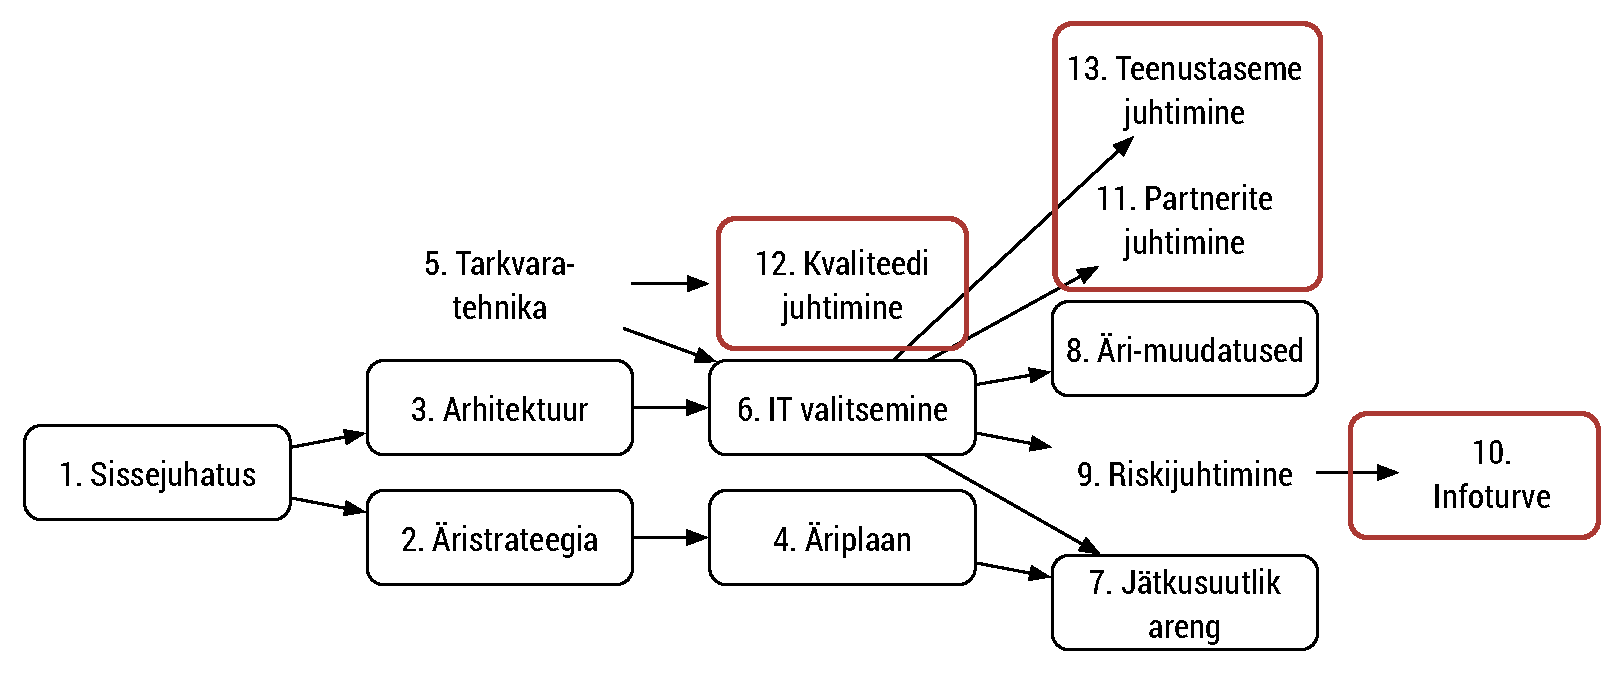
\includegraphics[width=\textwidth]{aine_struktuur_neljas.pdf}
\end{frame}

\section{Infoturve}
\begin{frame}[fragile]
  \frametitle{Küberründe võrratus}
	\begin{center}
	  Rünne tasub end ära siis ja ainult siis, kui:\par
		$S_p>P_f(S_a + P_c S_c)$
	\vfill
	\begin{description}
		\item[$S_p$] Ründest oodatav kasu
		\item[$P_f$] Ründe ebaõnnestumise tõenäosus
		\note{Ründe ebaõnnestumise tõenäosus on reaalselt alati väiksem kui üks: küsimus ei ole sisse saamises, küsimus on kiiruses, hinnas ja sügavuses. Kui otse rünnatakse, siis ka maha võetakse\par}
		\item[$S_a$] Ründe läbi viimise kulu
		\item[$P_c$] Vahele jäämise tõenäosus
		\item[$S_c$] Vahele jäämise kulu
	\end{description}
	\note{Selle valemi juures on oluline mõista, et tegu on alati ründaja poolt antud hinnanguga, järelikult on oluline osa probleemist avalikkussuhted ja avalikkusele kontrollitud mulje jätmine nii oodatavast kasust, õnnestumistõenäosusest kui vahele jäämise tagajärgedest ning tõenäosusest\par}
	\end{center}

\end{frame}

\begin{frame}[fragile]
  \frametitle{Muutujate seis}
	\begin{itemize}
		\item $S_p$ kasvab, kuna 
			\begin{itemize}
				\item Andmeid saab kasutada (ka) järgmise rünnakute jaoks (tagasiside) 
				\item Interneti sõltuvus reklaamist ja seega privaatsest infost kasvab
				\note{Maailmas investeeritakse aastas ca \$30 miljardit VC raha tarkvaraärisse. See peab kuskilt tagasi tulema. AId nõuavad samuti toitmist\par}
				\item Eksisteerib toimiv andmete ja ründeteenuste must turg
			\end{itemize}
		\item $P_f$ kahaneb, kuna süsteemid lähevad järjest keerulisemaks
		\item $S_a$ on dramaatiliselt langenud, kuna 
			\begin{itemize}
				\item Ründed on paljus automatiseeritud
				\item Ründevahendid on \emph{commodity} ja odavnevad seega kogu aeg
				\item Toimib tagasiside: mida rohkem arvuteid üle võetakse, seda rohkem arvuteid suudetakse rünnata ja seega ka üle võtta
			\end{itemize}
		\item $P_c$ arenenud riikides kasvab, mujal stabiilne
		\item $S_c$ arenenud riikides kasvab kiiresti (vt. megauploadi juhtum)
	\end{itemize}
	\note{Võrratuse parem pool kahaneb, kuna ründed lähevad odavamaks ja efektiivsemaks palju kiiremini, kui kasvab vahele jäämise tõenäosus. \par Sc väga palju kasvatamine enam ei õnnestu, ühiskond ei seedi ära väga suurt vahet mõrvari ja häkkeri karistuste vahel.}
\end{frame}


\begin{frame}[fragile]
  \frametitle{Võrratuse järelmid}
  	\begin{itemize}
		\item Järjest rohkem rünnakuid tasub ennast ära
		\item Üksikud intsidendid on asendunud pideva vooga
	\begin{itemize}
		\item Põhjuseks rünnete hinna langemine kiiremini, kui suudetakse tõsta vahele jäämise kulusid ja tõenäosust
		\item CERT-EE hinnagul ei ole praeguseks \emph{(spear) phishingu} kampaaniate vahel enam pause. Tegu on pideva survega
		\item Väga suurt rolli mängib automatiseerimine: kuigi automatiseeritud või \emph{drive-by} ründe $P_f$ on suhteliselt suur, on $S_a$ sisuliselt null
	\end{itemize}
	\end{itemize}
\end{frame}

\begin{frame}[fragile]
  \frametitle{Turvalisus ja arhitektuur}
	\begin{center}
		Ohutus (turvalisus) ei ole mitte süsteemi funktsioon vaid selle emergentne käitumine
		\note{Sotsiotehniline süsteem! Turvalisust ei saa funktsionaalsete nõuete kaudu väljendada. Saab nõuda teatud testide läbi viimist ja saab püstitada ohutusnõuded, kuid ohutust kui sellist ei saa ei nõuda ega testida. Turvalisus on olemuslikult operatiivne nähtus.}
	\end{center}
	\cite{leveson2011engineering}
\end{frame}

\begin{frame}[fragile]
  \frametitle{Turvalisus tuleb arhitektuurist}
	Turvalisus peab olema sisse ehitatud süsteemi arhitektuuri
	\begin{itemize}
		\item Seda ei saa hiljem lisada ega "külge kruvida"
		\item Kuna me ei suuda emergentsust kontrollida, on turvalisuse tagamine süsteemi elutsüklit läbiv protsess: Ohuanalüüsi tulemid on sisendiks disainiotsustele mis realiseerituna omakorda annavad sisendi uuele ohuanalüüsile
		\item Olulisel kohal on süsteemi kontseptsioon: kas idee on toetuda ühe sõlme turvalisusele või on terve süsteem ehitatud vastupidavaks?
		\note{Lõuna-Korea isikukoodi näide\par}
	\end{itemize}
\end{frame}

\begin{frame}[fragile]
  \frametitle{Infoturbe strateegiast}
	Mõned infoturbe strateegilised aspektid:
	\begin{itemize}
		\item Tuleb määratleda ja kommunikeerida aktsepteeritud riskitase 
		\note{Kuigi nuga on ohtlik, on ta meil siiski enamasti olemas. Kasulikkus kompenseerib riski\par}
		\item Peab eksisteerima koostöö PRi ja infoturbeinimeste vahel
		\begin{itemize}
			\item Ründaja käitumine sõltub väga paljus kuvandist
			\note{PRi kohta vt. märkmetest. Ründaja peab oma võrratuse parameetreid kuidagi hindama, seda hinnangut saab soovitud suunas mõjutada läbi kommunikatsiooni\par}
			\item PR tegeleb (kriisi) kommunikatsiooniga
		\end{itemize}

		\item Strateegiline roll on kogukonnal:
		\begin{itemize}
			\item Süsteemi olulised komponendid ei ole tingimata teie kontrolli all
			\item Tundliku info jagamise aluseks on usaldus
			\note{Õige käitumise aluseks on õigeaegne info\par}
			\item Internet on üksi hakkama saamiseks liiga terviklik süsteem
			\note{CERTide võrk tekkis üsna kohe pärast internetti\par}
			\item Panustage ja te saate vastu
			\note{Teie infoturbevõimekus peab olema pisut üledimensioneeritud tagamaks sotsiaalse krediidi taastootmist. Küberkaitseliit ja muud kogukondlikud ettevõtmised. Selle eelduseks on, et teil on inimesed, kes on suutelised reaalselt panustama\par}
		\end{itemize}

	\end{itemize}
\end{frame}


%Arutelu koht
\begin{frame}[fragile]
  \frametitle{Arutelu koht}
		\begin{center}
			\textbf{Kuidas tellida turvalist tarkvara?}
		\end{center}
\end{frame}


\section{Partnerite juhtimine}
\begin{frame}[fragile]
  \frametitle{Eetikast}
	\begin{center}
		Enne igasugust partneritega tegelemist veendu, et võtmeisikute arusaamad eetikast omavahel kattuvad ning mahuvad kõik mugavalt seaduse raamesse 
		\note{Kohtumine julgeolukuorganitega on pehmelt öeldes ebameeldiv ka siis, kui sa õigeks jääd. Ja kriminaalasi kindlasti mitte ei kiirenda tarkvara valmimist. Eetika pinnalt tekkinud väärtuskonflikt on samuti väga ebameeldiv ja tavaliselt ajakavale hukatuslik.}
	\end{center}
\end{frame}

\begin{frame}[fragile]
  \frametitle{Eesmärkidest}
	\begin{center}
		Teil on partneriga põhimõtteliselt vastuolulised eesmärgid. \par Harjuge ära, ärge võtke isiklikult ja õppige sellega elama
		\note{Oluline on leida ajas piiratud ühine komplekt eesmärke. Partneri motiveerimine. \par Siin tuleb mängu strateegia dünaamika: me mängime alati mängu (mänguteooria viide) partneriga. It takes two to tango}
	\end{center}
\end{frame}


\begin{frame}[fragile]
  \frametitle{Strateegiline posistioon}
  	Partnerit saab juhtida vaid sobivalt strateegiliselt positsioonilt	
	\note{Oma tahet saab peale suruda kas siis, kui olete tugevam, kui suudate olla nutikam või kui suudate paremini manööverdada. Ja teie partner seda kõike parasjagu ei suuda. \par}
	\begin{itemize}
		\item Tuletage meelde Sun Tzud
		\note{... kes teab, kuidas toimida tugevama ja nõrgema vastasega\par}
		\item Partneril tegeleb reeglina teiega kliendihaldur, kes keskendub vaid teile. Teil on reeglina mitu partnerit
		\note{Tihti on tegemist profiga või nende tiimiga. Hästi makstud oskajad inimesed\par}
		\item Ka väga suured riigid ei suuda enam suurkorporatsioonidele vastu seista \citep{partner}
		\item Ärge tehke endale illusioone oma võimete osas!
		\note{Eestis on vast kaks suuremat panka suutelised suuremaid teenusepakkujaid juhtima}
	\end{itemize}
		\note{Igivanas dilemmas jõu ja mõistuse kasutamise osas strateegias olete te (eriti avalikus sektoris) reeglina nõrgemal poolel. Te peate suutma kasutada mõistust.}

\end{frame}


\begin{frame}[fragile]
  \frametitle{OODA (VAOT) tsükkel}

	\begin{center}
		\includegraphics[width=\textwidth]{OODA.Boyd.svg.png}\\
		  	©Patrick Edwin Moran. Tsüklis tuleb liikuda vastaspoolest kiiremini muutes vastasel õige tegutsemise võimatuks. Olukord muutub enne, kui tsükkel läbitakse.
			\note{Riigiasutusel ei ole mõeldamatu liikuda kiiremini end täis söönud partnerist. Turult on näiteid olemas}
	\end{center}
\end{frame}

\begin{frame}[fragile]
  \frametitle{Toimimisest}
	\begin{center}
		\begin{quote}
	toimi toimimata\\
	ning ei ole nii\\
	et ei oleks juhtimist
   		\end{quote}
	\end{center}
\cite{laozi}
\end{frame}

\begin{frame}[fragile]
  \frametitle{Toimida toimimata}
	\begin{center}
			Kuidas vältida vajadust partnereid juhtida?
			\vfill
			Järgnevas mõned strateegilised võimalused selleks
	\end{center}
	\note{Võib ka vaadata nii, et järgneva abil tekitate endale strateegilise positsiooni}
\end{frame}


\begin{frame}[fragile]
  \frametitle{Tee mittejuhtimiseni}
	\textbf{Ignoreeri kogu probleemi}
	\begin{itemize}
		\item Mis vahet seal on, kes ja kuidas tarnib kohvi ja pastakaid?
		\note{Kuni hind on vähegi mõistlik. Ja kui enam ei ole, siis tarnib keegi teine. Jällegi küsimus olukorrast turul ja kontektist\par}
		\item Nii te ei saa täpselt seda, mida te tahate
		\note{Aga kohvi puhul reeglina ei ole oluline saada täpselt seda, mida tahetakse}
		\item Võib keskenduda ka lihtsalt koostöös parima tulevuse saavutamisele, jättes strateegilised mängud kõrvale
	\end{itemize}
\end{frame}

\begin{frame}[fragile]
  \frametitle{Tee mittejuhtimiseni}
		\textbf{Juhi tehnoloogiat}
	\begin{itemize}
		\item Selle asemel et juhtida partnereid, keskendu oma tehnoloogilise baasi kontrollimisele
		\item Kui kogu IP, arhitektuursed otsused, haldus jne. on teie käes, ei ole palju vahet, kes musta tööd teeb
		\item See kitsendab koostöömudeleid:
		\begin{itemize}
			\item \emph{Time-and-material}
			\item Väga põhjalikult spetsifitseeritud rangelt tehnilised tööd
		\end{itemize}
		\item Mõistlik valik, kontroll tehnoloogia üle on enamasti hea idee
		\item Eeldab tehnilise kompetentsi olemasolu majas
	\end{itemize}
\end{frame}

\begin{frame}[fragile]
  \frametitle{Tee mittejuhtimiseni}
		\textbf{Juhi ja/või kasuta standardeid}
	\begin{itemize}
		\item Selle asemel et juhtida partnereid, kasuta avatud standardeid, vajadusel kirjuta uued
		\item Kui kogu tegevus on standardipõhine, on partneri vahetus suhteliselt lihtne ja valutu
		\item Eriti kasulik kombinatsioonis "jaga ja valitse" strateegiaga
		\item Töömahukas
		\note{Töömahukas, kui sobivaid standardeid ei ole}
	\end{itemize}
\end{frame}

\begin{frame}[fragile]
  \frametitle{Tee mittejuhtimiseni}
	\textbf{Juhi kogukonda}
	\begin{itemize}
		\item Ühe partneri juhtimise asemel tekita isereguleeruv seltskond 
		\item Osavalt käima lükatud kogukond hoiab end ise püsti
		\item Jälle kasulik koos "jaga ja valitse strateegiaga"
		\item Keeruline teha kuid kuldne, kui käima läheb
		\item Väga paljud \emph{open-source} asjad käivad nii, tegu on suhteliselt hästi tuntud praktikaga
		\note{Mis te arvate, miks vähegi asjalikumad sisemised tööriistad tänapäeval open source on (Ghibli näide)? Sest kaotada ei ole suurt midagi aga võita on suur kogukond}
	\end{itemize}
\end{frame}

\begin{frame}[fragile]
  \frametitle{Strateegilised valikud}
	\textbf{	Jaga ja valitse}
	\begin{itemize}
		\item Jaga oma süsteem rangelt piiritletud komponentideks 
		\item Iga komponent eraldi hanke/hoolduse/uuenduse subjektiks
		\item Piirijoontel kasuta standardeid või rangelt kontrollitud liideseid
		\note{Ka protsessiliidesed (relase!)}
		\item Näiteks: andmehoidla ja rakendusserver on eraldatud S3\footnote{\url{http://aws.amazon.com/s3/}} abil
		\item Hüved:
		\begin{itemize}
			\item Ühelgi partneril ei ole kontrolli terve süsteemi üle
			\item Et liidesed on igal juhul paigas, võib tarnijaid lihtsasti vahetada
			\item Modulariseerimine on igal juhul hea mõte
		\end{itemize}
		\item Vajab tehnilist- ja protsessikompetentsi, töömahukas
	\end{itemize}
\end{frame}


%Arutelu koht
\begin{frame}[fragile]
  \frametitle{Arutelu koht}
		\begin{center}
			\textbf{Kuidas vabaneda end sisse söönud "puugist"?}
		\end{center}
\end{frame}

\begin{frame}[fragile]
  \frametitle{Partnerite juhtimine}
  Kui siiski on vaja partnerit juhtida
	\begin{itemize}
		\item Vali sarnane partner: suurus, ajahorisont, küpsusaste
		\note{Kerry King: Time is not a cool thing to waste\par Olukord, kus sellist saada ei ole, on ohu märk! Miks ei ole see teenus ostetav?\par}
		\item Käitu kehtestavalt: väljenda oma vajadusi selgelt ja järejekindlalt ning seisa nende eest
		\item Kaasa riskijuhid, partnerid on olulised riskide allikad
		\item Tee selgeks ökosüsteem
		\note{Kes on veel mängijad? Mis on nende huvid? vt. ka märkused seoste kaardistamine kohta\par}
	\end{itemize}
\end{frame}

\begin{frame}[fragile]
  \frametitle{Isiklik kogemus}
	\begin{center}
			\vfill
			Kui partner tundub rumala või pahatahtlikuna,\\ on reeglina põhjust peeglisse vaadata
			\vfill
			\note{Partnerist lahti saamine on reeglina ressursimahukam kui oma käitumise parandamine. Samas on ka praegu riigis sigimas olukord, kus ühes asutuses tahetakse vahetada partnerit soovimata muuta oma käitumist. \par Miks te arvate, te teise partneriga põhimõtteliselt teisiti läheb?}
	\end{center}
\end{frame}

\begin{frame}[fragile]
  \frametitle{Võtmeküsimus}
	\begin{center}
		Kuidas olla pädev klient?
		\note{It takes two to tango!\par Järgnevas levinumad strateegilised valukohad}
	\end{center}
\end{frame}

\begin{frame}[fragile]
  \frametitle{Kontroll IP üle}
  Oluline on saavutada kontroll tekkiva intellektuaalomandi üle
	\begin{itemize}
		\item Omand ei võrdu kontrolliga
		\note{Mu auto on liisingfirma oma aga tööle sõidan sellega mina\par}
		\item Kus tekib intellektuaalomand?
		\begin{itemize}
			\item Ehk: kus tekib väärtus?
			\note{Partnerluse kuldreegel: ära kunagi osta väljast väärtusloomet!\par}
			\item Tänapäeval ei ole tarkvara lähtekood reeglina omaette väärtus 
			\note{Järelikult ei ole kriitiline tarkvara lähtekoodi dokumenteerimine. X-tee oli võimalik kuue kuuga nullist uuesti kirjutada\par}
			\item Väga tihti sünnib väärtus kliendi juures
			\note{Teadmine äriprotsessist sünnib kliendi juures. Ärianalüütik võib kogu teadmisega minema kõndida!\par}
			\item Küsimus on teadmuses
			\note{Teadmust niisama lihtsalt paberi peal edasi ei anna, paberil liigub info ja need kaks ei ole sünonüümid\par}
		\end{itemize}

	\end{itemize}
	\begin{center}
		\emph{Intellektuaalomandit kontrollib see, \\kes kontrollib seda loovaid inimesi}
		\note{Mida rohkem sinu inimesi on võtmeotsuste juures, seda parem on sinu kontroll, sest intellektuaalomand tekib IT vallas inimeste peas\par}
	\end{center}

\end{frame}

\begin{frame}[fragile]
  \frametitle{Kontroll arhitektuuri üle}
  	Oluline on saavutada kontroll süsteemi arhitektuuri üle
	\begin{itemize}
		\item Tuletage meelde arhitektuuri seost ärimudeliga
		\note{Kui te ei kontrolli arhitektuuri, ei kontrolli te oma ärimudelit. Mis on, ütleme, halb\par}
		\item Kontseptsioon on tihedalt seotud väärtuste, mõttemallide ja seeläbi organisatsiooni kultuuriga
		\note{Arhitektuuri kontrollimata lasete te kellegi teise oma organisatsiooni kultuuri mõjutama\par}
		\item Partner lähtub lokaalsest optimumist (või enda omast)
		\note{Partner järgib lokaalset optimumi, teie roll on arendada terviklikku süsteemi arhitektuuri\par}
		\item Võõraste väärtuste ja mõttemallide üle võtmine on väga raske. 
		\begin{itemize}
			\item Ka siis, kui need on peidetud arhitektuuri
			\item Vajadus võtta üle tellija mõttemall tasandab mänguvälja
			\note{Vajaduse kelle iganes mõttemalli üle võtta tõstab hinda! Valikukoht!\par}
		\end{itemize}
		\note{Seetõttu ongi arendaja vahetamine reeglina keeruline: igaühel on oma juurdunud viis asju ehitada ja ümber harjumine on keeruline/kallis}
	\end{itemize}
\end{frame}

\begin{frame}[fragile]
  \frametitle{Kontroll suhte üle}
  	Kelle käes on initsiatiiv suhetes partneriga?
	\begin{itemize}
		\item Kõik algab kontrollist lepingu üle
		\begin{itemize}
			\item Tuletage meelde juttu keerukusest
			\note{Natuke kihtsamaid asju on palju lihtsam kontrollida\\}
			\item Iga lepingusse kirjutatud punkt on täitmiseks
			\note{Kunagi ei tohi lepingusse kirjutada asju, mida te "võib olla" jõustate\par}
			\item Kui teie ei suuda lepingut täita, ärge oodake seda ka partnerilt
			\item "Kui me ei täida punkti x, miks peaksime täitma punkti y?"
			\item "Punktis a me tulime ju teile vastu, tulge teie vastu punktis b"
		\end{itemize}
		\item Erilise tähelepanu all olgu suhetele suuantud protsessid, rutiinid, tegevused
		\note{Suhetele suundatud asjade puhul on kriitiline kliendi mõjutamine korrektselt käituma. Vastasel juhul jääte kahe tule vahele: rahul ei ole ei klient ega partner\par}
		\begin{itemize}
			\item Tellimuste esitamine
			\note{Kasutuslugude esitamine nihkub kaks nädalat aga lõpptähtaeg jääb paika. Päriselt või?\par}
			\item Muudatuste juhtimine ja skoobi kontroll
			\item Vastuvõtutestid
			\item Üle andmine ja vastu võtmine
		\end{itemize}
		\item Tuletage meele Sun Tzud
		\note{All warfare is based on deception\par}
		\item \emph{In God we trust, everybody else pays cash}
	\end{itemize}
\end{frame}

%Arutelu koht
\begin{frame}[fragile]
  \frametitle{Arutelu koht}
		\begin{center}
			\textbf{Mida saab teha saamatu kliendiga?}
		\end{center}
\end{frame}

\section{Kvaliteedi juhtimine}

\begin{frame}[fragile]
  \frametitle{Vigadest tarkvaras}
	Tarkvara on alati natuke katki, miks?
	\begin{itemize}
		\item Kui tehakse ühik tööd, võib see olla tehtud kas õigesti või valesti vajades ümber tegemist
		\item Valesti tehtud tööd ei avastata kohe, avastamiseks kuluv aeg sõltub vigade hulgast
		\item Vea parandamine on samuti ühik tööd, ka seda võib teha kas õigesti või valesti
	\end{itemize}
\end{frame}

\begin{frame}[fragile]
	\frametitle{Kui palju on tarkvaras vigu?}
	\vfill
	\begin{center}
		Kuidas kirjeldatud mudel käitub? 
		\note{Nelja muutujaga diferentsiaalvõrrandisüsteem. Laske käia!}
	\end{center}
	\vfill
\end{frame}


\begin{frame}[fragile]
  \frametitle{Projekti mudel}
  	\begin{center}
			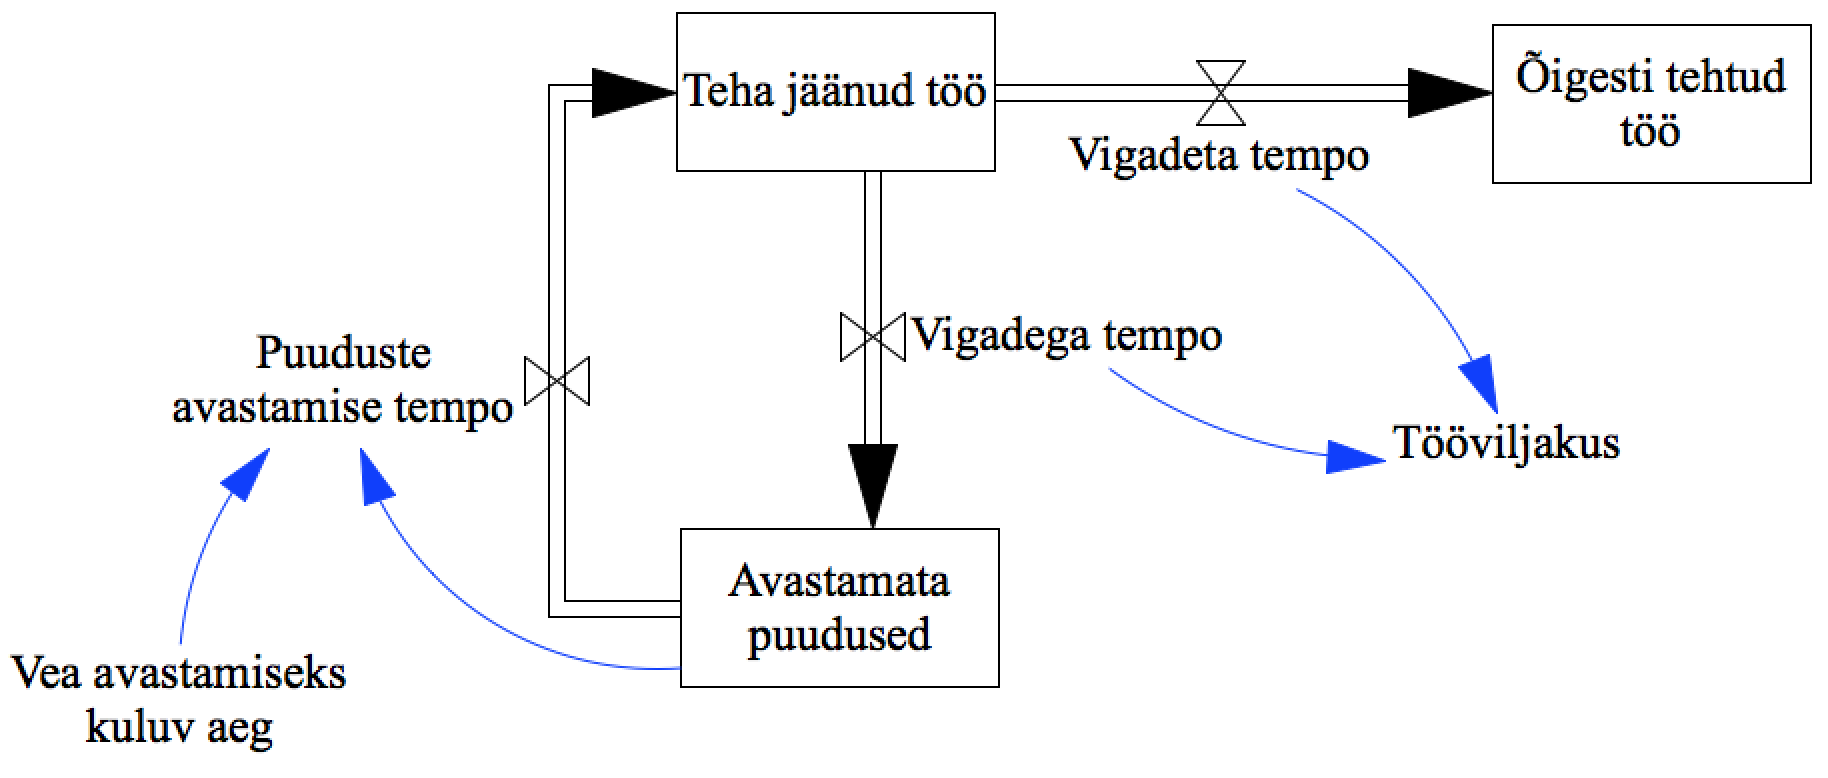
\includegraphics[width=.9\textwidth]{vead_mudel.png}
	\end{center}
\end{frame}


\begin{frame}[fragile]
  \frametitle{Mudeli simuleerimise tulemus}
  	\begin{center}
			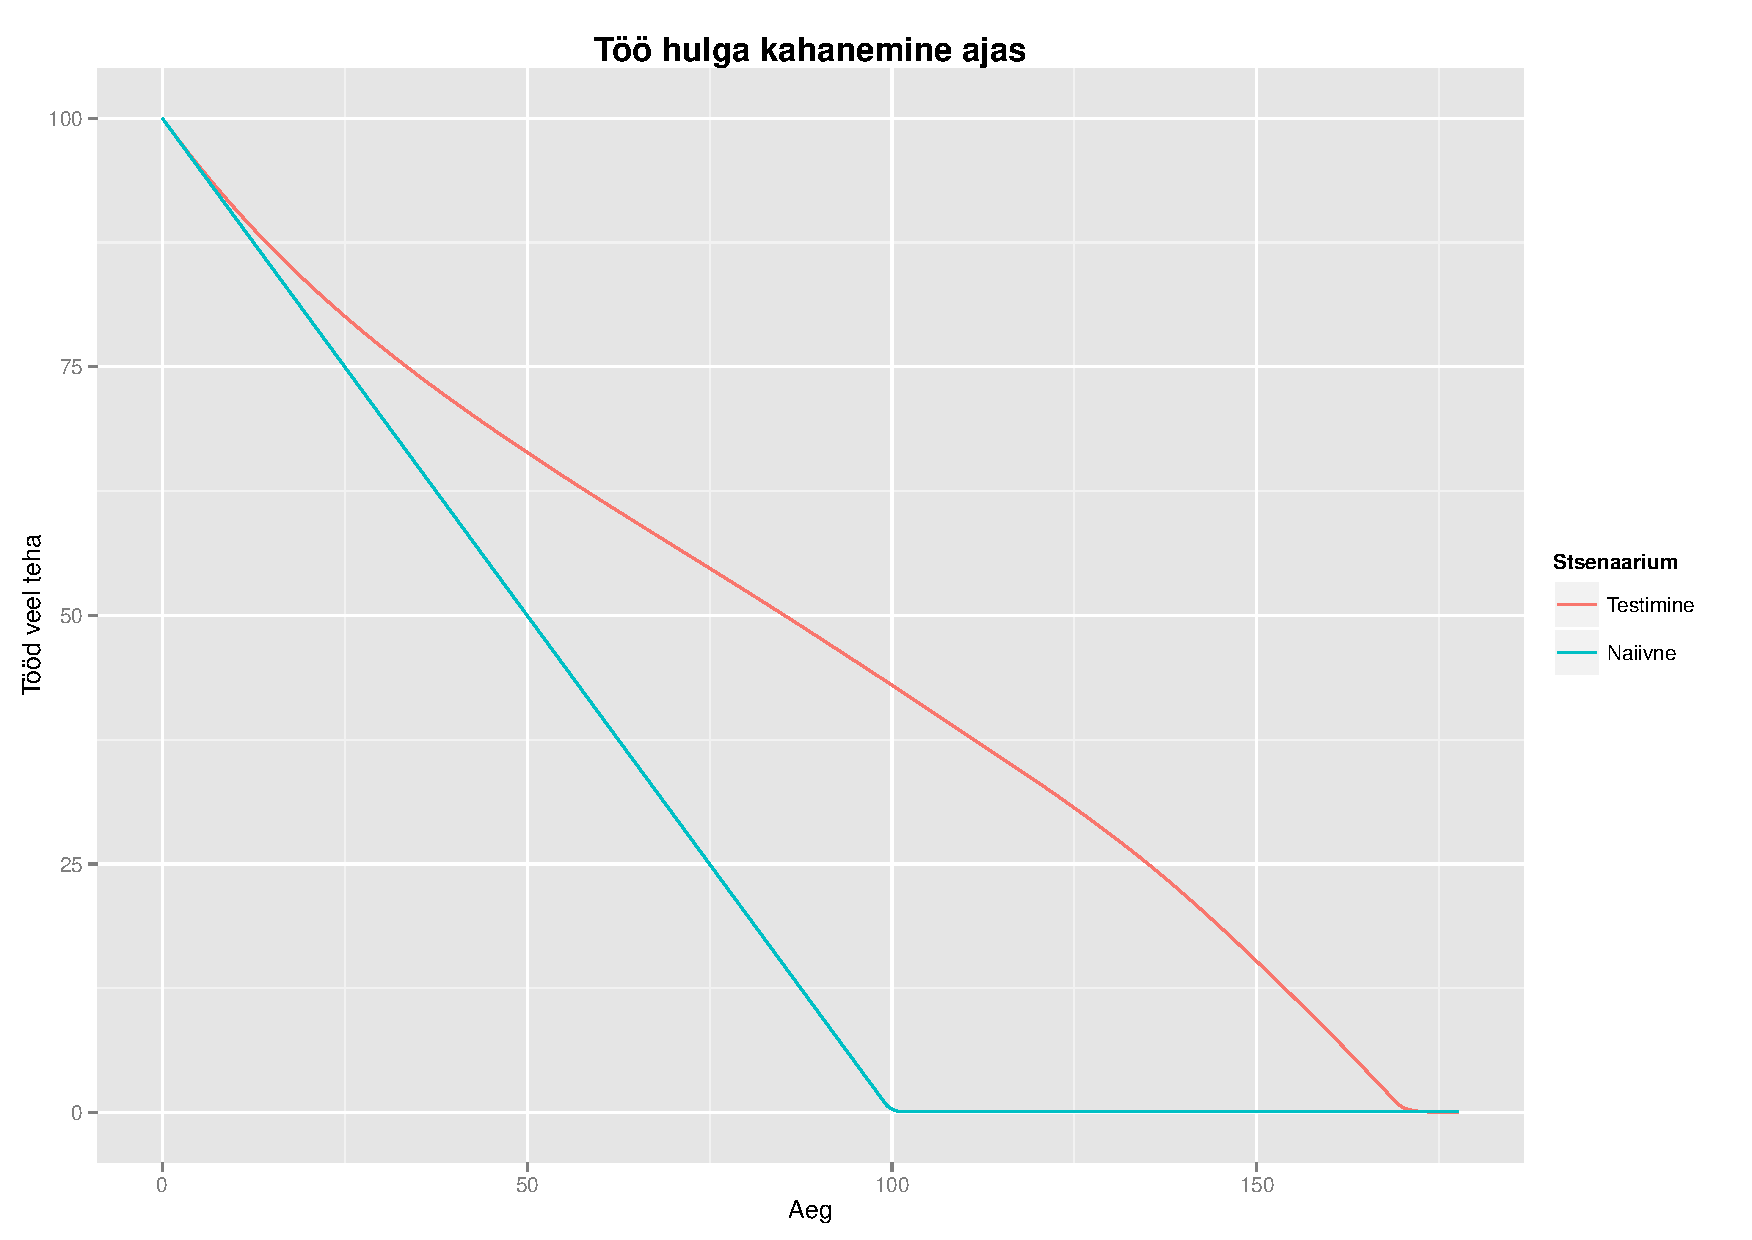
\includegraphics[width=.9\textwidth]{vead.pdf}
	\end{center}
\end{frame}

\begin{frame}[fragile]
  \frametitle{Vaatame lähemalt}
  	\begin{center}
			\includegraphics[width=.9\textwidth]{vead_zoom.pdf}
	\end{center}
\end{frame}


\begin{frame}[fragile]
  \frametitle{Järeldused}
	\begin{itemize}
		\item Erinevus naiivsest mudelist on ligi kaks korda!
		\item Graafiku kuju on ka lihtsa mudeli puhul mittetriviaalne ning intuitiivselt raskesti hinnatav
		\item Lõpuks hakkab graafik kahanema eksponentsiaalselt
		\note{Eksponent aga ei jõua kunagi nulli}
	\end{itemize}
	
\end{frame}

\begin{frame}[fragile]
	\frametitle{Oluline järeldus:}
	\vfill
	\begin{center}
		Tarkvaras on alati vead  
	\end{center}
	\vfill
\end{frame}

\begin{frame}[fragile]
  \frametitle{Strateegilised implikatsioonid}
	\begin{itemize}
		\item On oluline määratleda, millal lõpetada testimine
		\note{On oluline testimise lõpp määratleda, sest puhta rakenduseni ei jõuta eales\par}
		\begin{itemize}
			\item Järelikult peab eksisteerima toimiv veahaldus koos hooldus- ja hindamisprotsessiga
			\item Peab arvesse võtma spetsifikatsiooni täpsust: ei ole mõtet testida detaile, mida spetsifikatsioonis ei ole
		\end{itemize}
		\item Testimine peab algama võimalikult vara
		\note{Kui testimist alustada hiljem, jääme liiga kauaks naiivset mudelit uskuma\par}
		\item Testimisprotsess kui selline on väga oluline
		\note{Testimisprotsessi ülesehitusest sõltub graafiku kuju\par}
	\end{itemize}
	
\end{frame}


%Arutelu koht
\begin{frame}[fragile]
  \frametitle{Arutelu koht}
		\begin{center}
			\textbf{Millal on tarkvara valmis?}
		\end{center}
\end{frame}

\begin{frame}[fragile]
	\frametitle{Kuidas suhtuda vigadesse}
	\vfill
	\begin{center}
	\begin{quote}
		High velocity organizations are constantly experimenting and learning more about all the work they do;\dots; These organisations do not encourage or admire workarounds, firefighting and heroic measures. They want to understand and solve problems, not put up with them.
		\note{"Tahetakse parimat, välja kukub nagu alati" suhtumine on suurepärane näide sellise suhtumise vastandist}
		\end{quote}
	\end{center}
	\cite{spear2010high}
\end{frame}

\begin{frame}[fragile]
  \frametitle{Lean \& QA}
	Moodsa kvaliteedijuhtimise juured on Toyotas\footnote{Täpsemalt, \emph{Toyota Production System, TPS}}, kus kasutatavat lähenemist tootmisele alates 90ndatest tuntakse ka kui \emph{"lean manufacturing"}  

	\begin{itemize}
		\item \emph{Lean} tootmise üheks aluseks on jäätmete ja raiskamise vältimine
		\note{Kõik jäätmete tüübid on tihedalt seotud ja põhjustavad üksteist\par}
		\begin{description}
			\item[Muda] Töö, mis ei lisa väärtust
			\note{Muda. Valesti tehtud töö ei lisa väärtust, samuti üleliigsed liigutused või sisutute paberite tootmine. Aga ka ootamine. Kokku seitse klassikalist muda\par}
			\item[Muri] Ebamõistlik töö
			\note{Muri. Kui töötaja (või masin) surutakse oma võimete piirist välja, ei saa head tulemust tulla ning toimub raiskamine\par}
			\item[Mura] Ebamõistlik töövoog
			\note{Mura. Kui üksikud sammud kokku ei sobi, toimub raiskamine}
		\end{description}
		\item Kuna raiskamine on tihti seotud ebakvaliteetse tootega, on \emph{lean} kvaliteedijuhtimisega tihedalt seotud
		\item Efektiivselt toimiv tootmisprotsess annab kvaliteetset tulemust
		\item Ka agiilsete meetodite juured on autotööstuses, väga paljus jagatakse mõtteviisi
	\end{itemize}
\end{frame}

\begin{frame}[fragile]
	\frametitle{Oluline järeldus:}
	\vfill
	\begin{center}
		Moodsa kvaliteedijuhtimise juured on efektiivsemas tootmises,\\ mitte lõppkasutaja rahulolus
		\note{ITs keskendub QA tihti vaid lõppkasutajale ning ei saa seega olla edukas. CI peaks olema QA, mitte programmeerijate ajada\par Seega seob moodne kvaliteedijuhtimine põhjuse otseselt tagajärjega: kui sant lõpptulemus võib, kuid ei pruugi, viia väiksema müügini (NSVL! Ja müük!=kasum!) siis raiskamine tootmises viib kindlasti väiksema kasumini}
	\end{center}
	\vfill
\end{frame}

\begin{frame}[fragile]
	\frametitle{Teine oluline järeldus:}
	\vfill
	\begin{center}
		Testimise ülesanne on hinnata süsteemi kvaliteeti
		\note{Sotsiotehnilise süsteemi! Lihtsalt speki vastu valideerimine on vaid osa rehkendusest}
	\end{center}
	\vfill
\end{frame}


\begin{frame}[fragile]
	\frametitle{Definitsioon: kaizen}
	\vfill
	\begin{center}
	\begin{quote}
		\dots kaizen (improvement), a process of engaging those closest to the direct work of the organization in the continual improvement of that work.
	\end{quote}
	\end{center}
	\cite{spear2010high}
\end{frame}

\begin{frame}[fragile]
  \frametitle{Kaizenist}
	Kaizen on üks mitmest viisist kvaliteedist mõelda. Selle definitsioonil on järgmised olulised osad:
	\note{Mitte, et ma oleksin mõnda teist kasutuses näinud. Aga kindlasti on näiteks brittidel oma viis asjadest mõelda.\par Me ei jõua väga sügavale detaili minna, see asi on palju keerulisem, kui paistab ja siin rääkida jõuab.\par}

	\begin{itemize}
		\item Kvaliteet tuleneb tööd otseselt tegevast inimesest
		\note{Kui programmeerija ei hooli oma töö tulemusest (või ei suuda seda tagada), ei saa süsteem olla kvaliteetne\par}
		\item Kvaliteedi juhtimine on süstemaatiline protsess
		\note{Kvaliteedi juhtimine ei seisne üle aia visatud koodi valideerimises kellegi arvamuse vastu süsteemi käitumisest\par}
		\item Kvaliteedi juhtimine on pidev protsess
		\note{Kuna koodis on definitsiooni järgi alati vead, ei lõpe kvaliteedi taga ajamine kunagi}		
	\end{itemize}
\end{frame}

\begin{frame}[fragile]
  \frametitle{Teede parandamisest}
    	\begin{columns}[t]
		\begin{column}[T]{4.5cm}
			\textbf{Tavapärane}
			\begin{itemize}
				\item Tees on auk 
				\item Auk parandatakse
				\item Auk tekib uuesti
				\item Auk parandatakse
				\item Auk tekib uuesti
				\item Auk parandatakse
				\item Auk tekib uuesti
				\item Auk parandatakse
				\item jne.
			\end{itemize}
		\end{column}
		\begin{column}[T]{6cm}
			\textbf{TPS}
			\begin{itemize}
				\item Tees on auk 
				\item Auk parandatakse
				\item Auk tekib uuesti
				\item Küsitakse "miks?"
				\item Leitakse vastus, auk parandatakse
				\item Auk tekib uuesti
				\item Küsitakse "miks?"
				\item Leitakse vastus, auk parandatakse
				\item Tee on korras
			\end{itemize}
		\end{column}
	\end{columns}
\note{Pange tähele seost jätkusuutlikkusega. Esimene viis on jätkusuutlik vaid lühikest aega (varem või hiljem on tees liiga palju auke, et neid parandada jõuaks), teine on jätkusuutlik, kuid ressursimahukam. Kui pikk on teie leping partneriga?}
  
\end{frame}

\begin{frame}[fragile]
  \frametitle{Järelmid IT QA-le}
	Kõigel sellel on järgmised järelmid IT QA kontekstis
	\begin{itemize}
		\item Kvaliteedi juhtimine peab olema ennekõike tarkvara tootja huvi
		\item Tarkvaratehnika peab olema pidevas arengus
		\note{Kui tarkvaratehnika ei muutu, ei saa õppimisprotsessi toimuda\par}
		\item Teadmusjuhtimisel on QAs oluline roll
		\note{Ilma teadmusjuhtimiseta ei saa toimuda õppimist, eriti õppimist teiste vigadest. Mida me oleme varem teinud olukorras, kus auk samasse kohta tagasi tuleb?\par}
		\item QA tiim peab olema programmeerijatele võrdväärne partner
		\note{Kui QA on lihtsalt seltskond, kes (paremal juhul) automaatteste kirjutab, ei suuda nad öelda, mida tarkvara tootmise protsessis teisiti teha. Ja kui ka oskaksid, ei võetaks neid tõsiselt\par}
		\item QA ei saa olla isoleeritud tegevus projekti lõppfaasis
		\note{Pidevast testimisest räägib ka meie eelnevalt kirjeldatud mudel\par}
	\end{itemize}
\end{frame}


%Arutelu koht
\begin{frame}[fragile]
  \frametitle{Arutelu koht}
		\begin{center}
			\textbf{Milline tarkvara on kvaliteetne?}
		\end{center}
\end{frame}


\section{Teenustaseme juhtimine}

\begin{frame}[fragile]
  \frametitle{Teenustaseme juhtimine}
	Teenustaseme juhtimise aluseks on 
	\note{Ilma nendeta ei ole mõtet rääkida teenuse juhtimisest. Kui kasvõi üks osis on puudu, teenust juhtida ei saa\par}
		\begin{itemize}
			\item Teenuse mõiste olemasolu organisatsiooni kõigis kihtides. Ehk, igal "teenusel" peab eksisteerima selgelt piiritletud
			\begin{itemize}
				\item tehniline komponent
				\item funktsioon
				\item organisatsiooniline vastutaja nii IT- kui tellija poolel
				\item äristrateegia- ja mõõdikud
			\end{itemize}		
			\item Reaalne motivatsioon teatava taseme kehtestamiseks
			\note{"Me hoolime sellest, kuidas meie kliendi kassil läheb" ei ole reaalne motivatsioon\par}
			\item Mehhanismi olemasolu käitumise korrigeerimiseks teenustaseme mittesaavutamisel
			\note{Taset ei ole mõtet mõõta, kui sellest miskit ei sõltu\par}
		\end{itemize}		
\end{frame}

\begin{frame}[fragile]
  \frametitle{Miks teenustaset juhtida?}
	\begin{center}
		Teenustaseme juhtimise aluseks on selgelt määratletud vajadus vältida teenuse taseme langemist alla teatud piiri
		\note{Pange tähele erinevust Kaizenist: seal räägitakse pidevast kvaliteedi ülespoole surumisest. Teenustase kui operatiivse süsteemi kvaliteet?}
	\end{center}
\end{frame}


\begin{frame}[fragile]
  \frametitle{Miks teenustaset juhtida?}
  	Teenustaseme langus alla teatud piiri ja sellest sündiv kahju on riski realiseerumise definitsioon
		\begin{itemize}
			\item Järelikult tuleb teenustaseme juhtimisest rääkida riskide kontekstis
			\item Vastasel juhul on tegu lihtsalt grupi jonnivate inimestega
			\note{Riskijuhtimine annab neile küsimustele ratsionaalse, mõõdetava ja rahasse valatava vastuse. Ilma riskijuhtimise mõtteviisita on sõna sõna vastu\par}
			\begin{itemize}
				\item Kui palju on väärt teenustaseme tõstmine X ühiku võrra?
				\item Milline on mõistlik teenustase?
				\item Mida tähendab "teenus ei ole kättesaadav"?
			\end{itemize}
			\item Riskijuthimine annab kvaliteeditaseme juhtimise strateegilise mõõtme 
		\end{itemize}		
\end{frame}

\begin{frame}[fragile]
  \frametitle{Teenuse mõõtmisest}
  	Mõõta ja hinnata tuleb teenust, mitte selle komponente
		\begin{itemize}
			\item Keerukate süsteemide puhul ei ole põhjus-tagajärg seos selge
			\note{Vähegi mittetriviaalse süsteemi puhul tekib lihtsasti olukord, kus kõik masinad on rohelised aga teenus on punane\par}
			\item Tõrke ajend võib olla mõõtmisvea piires
			\note{Tuletage meelde keerukuse definitsiooni: kuitahes väike muutus sisendis võib anda kuitahes suure muutuse väljundis\par}
			\item Mitte kõik süsteemi komponendid ei ole teie kontrolli all
			\note{Tuletage meelde juttu süsteemi piiridest. Tüüpiliseks näiteks on siin internetiühendus või näiteks Google. Kas teie teenus on kättesaadav, kui suurim ISP ei suuda nime lahendada ja teie domeen on Google blacklistis?\par}
			\item Masinate mõõtmine on ka suhteliselt mõttetu: riistvara vead on suhteliselt teadaoleva jaotusega sündmused
			\item Eriti oluline on teenusekesksus numbriliste mõõdikute korral
			\note{Veebilehe vasteaeg ei võrdu HTMLi serverist väljastamise ajaga. Tänapäeval väga keeruline teema (CDNid, eri DNSi pakkujad, pilvetehnoloogiad jne.). Ärge investeerige ilma selge vajaduseta, see teenus on võimalik sisse osta.\par}
			\item Strateegiliselt on oluline vaadata teenuse kvaliteeti kui tervikut eristamata tehnilist komponenti
			\note{Ehk, teie süsadmine peaks mõõtma NPSi abil.}
		\end{itemize}		
\end{frame}

\begin{frame}[fragile]
  \frametitle{Oluline}
	\begin{center}
		Teenuse monitooring on oma olemuselt analüütikaprobleem
		\note{Suure koguse logide, servierinfo ja muu pealt tuleb teha otsus teenuse hetkelise kättesaadavuse kohta. Täiesti mittetriviaalne, eriti kui majas puudub BI võimekus}
	\end{center}
\end{frame}


\begin{frame}[fragile]
  \frametitle{Modelleerimisest}
	On oluline panna vastu kiusatusele modelleerida süsteemi tõrkeid leidmaks seost serveri ja teenuse tõrke vahel
	\note{Strateegiliselt väga riskantne samm. Räägin, sest olen seda kiusatust palju näinud ka mõistlike inimeste puhul\par}
		\begin{itemize}
			\item Võib tekkida kiusatus siduda organisatsiooni eri taseme mudelid
			\note{Kui kõik neli on olemas, saame riistvaravea viia läbi konfiguratsioonihalduse arhitektuurimudelini, kust paistab välja mõjutatud teenus\par}
			\begin{itemize}
				\item Monitooringu mudel
				\item Konfiguratsioonihalduse mudel
				\item Tarkvara arhitektuuri mudel
				\item Teenuste mudel
			\end{itemize}
			\item Ärge seda palun ilma mõjuva põhjuseta tehke:
			\note{Mudelite sidumist võib kaaluda, kui eesmärk on selge ning nõutav panus on miskipärast (kõik neli mudelit on ühe tootja tarkvaras) väike\par}
			\begin{itemize}
				\item Põhjus-tagajärg seostest juba rääkisime
				\item Nagu ka kõik-on-kogu-aeg-nii-kui-nii-katki reaalsusest
				\item Nii muutuvad kõik neli mudelit eesmärgiks ja mitte vahendiks
				\note{Saba hakkab liputama koera\par}
				\item Organisatsiooni lisandub väga palju kaheldava väärtusega keerukust
			\end{itemize}
			
		\end{itemize}		
\end{frame}

%Arutelu koht
\begin{frame}[fragile]
  \frametitle{Arutelu koht}
		\begin{center}
			\textbf{Mis on teenus?}
		\end{center}
\end{frame}


\section{Viited}

\begin{frame}[t,allowframebreaks,]
  	\bibliographystyle{plainnat}
	\bibliography{it_strateegia} 

\end{frame}

%\plain{Küsimusi?}
\begin{frame}[plain]
	\begin{center}Küsimusi?\end{center}
\end{frame}


\end{document}